\chapter{Background}
\label{ch:background}

% Your literature review goes here. \citet{hughes1989functional} discusses the advantages of functional programming by exploring \emph{e.g.}\ lists, trees, and noughts and crosses in a functional programming language. 
\section{Topic Modelling}\label{sec:topic_modelling}
As discussed in \Cref{ch:introduction}, this project uses topics to identify what the posts are about. This section will discuss
how topics are created and how they are used in this project.\\
There are 2 methods of topic modelling that were considered for this project. The first method is Unsupervised Learning, and the
second method is Supervised Learning.\\
\subsection{Unsupervised Learning}
Unsupervised learning is a method of machine learning that does not require labelled data. This method is used to identify patterns
in data \cite{mahesh2020machine}. For this project, the patterns are topics.\\
Using gensim LDA \cite{gensimLDA} with pyLDAvis \cite{LDAVis}, and BERTTOPIC \cite{BERTTopic}, topics were identified from a set of unlabelled documents.
\newpage
\begin{figure}[hbtp]
    \centering
    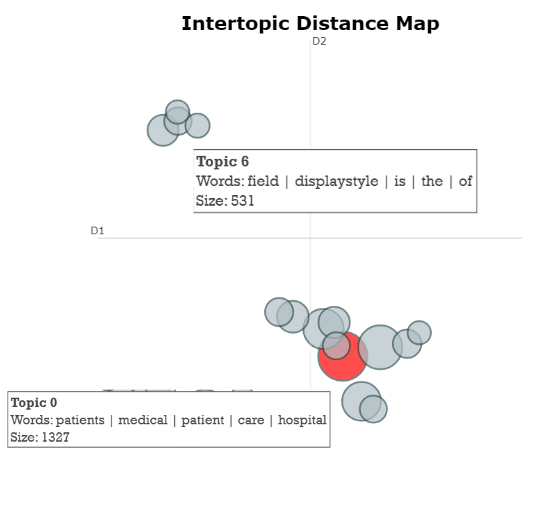
\includegraphics[width=0.6\textwidth]{../images/ldatopic.png}
    \caption{LDATopic creating topics from a set of unlabelled documents}
    \label{fig:ldatopic}
\end{figure}

The benefits of using unsupervised learning are that it does not require labelled data \cite{mahesh2020machine}, it is easy to implement, and the classification
of posts with the generated topics should be accurate - as the topics are generated to be separable. The downsides of using unsupervised
learning are that the topics generated may not be meaningful; Take for example Topic 6 from \Cref{fig:ldatopic}. This topic is made up
of the words `displaystyle', `is', `the', and `of'. It is quite hard for a human to understand what this topic is about.

\subsection{Supervised Learning}\label{sec:supervised-learning}
Supervised learning is a method of machine learning that requires labelled data. The labelled data acts as a teacher to the model, and
the model learns from the labelled data \cite{mahesh2020machine}.\\
For this project, a set of topics can be manually created and then used to label the posts. This method is much easier to implement
than unsupervised learning, as the topics are already created. The downside of this method is that it requires labelled data, which
can be time consuming to create.\\

For this project, supervised learning was used to classify the posts into the topics that were created. The original set of topics were:
\begin{multicols}{2}
\begin{itemize}
    \item \textbf{Culture}
    \item \textbf{Entertainment}
    \item \textbf{News}
    \item \textbf{Philosophy}
    \item \textbf{Religion}
    \item \textbf{Science}
    \item \textbf{Sports}
    \item \textbf{Technology}
    \item \textbf{Law}
    \item \textbf{History}
    \item \textbf{Geography}
    \item \textbf{Video Games}
    \item \textbf{Music}
    \item \textbf{Medicine}
    \item \textbf{Business}
    \item \textbf{Foods}
    \item \textbf{Disasters}
    \item \textbf{Nature}
    \item \textbf{Education}
    \item \textbf{Politics}
    \item \textbf{Economics}
    \item \textbf{Computer Science}
    \item \textbf{Mathematics}
\end{itemize}
\end{multicols}

Pythia \cite{Pythia} gave inspiration for most of the topics. Some extra topics were included to deal with uncovered topics, such as
`Video Games' and `Foods'.\\

Once the topics were created, labelled data was created using a distant supervision method. Using Subreddits and Wikipedia categories
as ground truth labels, and posts within those Subreddits and Wikipedia categories as the data. The labelled data was then used 
to train a supervised learning model. Although distant supervision allows us to quickly create labelled data, it is not perfect. 
The ground truth labels may not be accurate, and the posts may not be relevant to the topic. This is due to the fact that the posts
can be made by anyone and it is possible that someone may post something that is not relevant to the Subreddit or Wikipedia category they
are posting in.
\section{Text Classification}

As mentioned in \Cref{ch:introduction} there exists research on topic identification in short texts such as social media posts.
Topic analysis on short posts is harder than on longer texts because of the lack of context \cite{DeepShortText}; Twitter posts are limited to 280
characters \cite{developers_counting_nodate}, so users tend to attach images, or reference other tweets (via retweeting) to add context that would not be obvious from
the text alone.



\subsection{Recurrent Neural Networks (RNN)}\label{sec:RNN}
Recurrent Neural Networks (RNNs) are Neural Networks that are used to model sequential data \cite{rnn-seq}. They are good at modelling sequential data
because they can take into account the previous inputs in the sequence when making a prediction. This makes them good for text
as the text input can be seen as a sequence of words and we can leverage the previous words to make a prediction about the whole sentence.\\
\begin{figure}[hbtp]
    \centering
    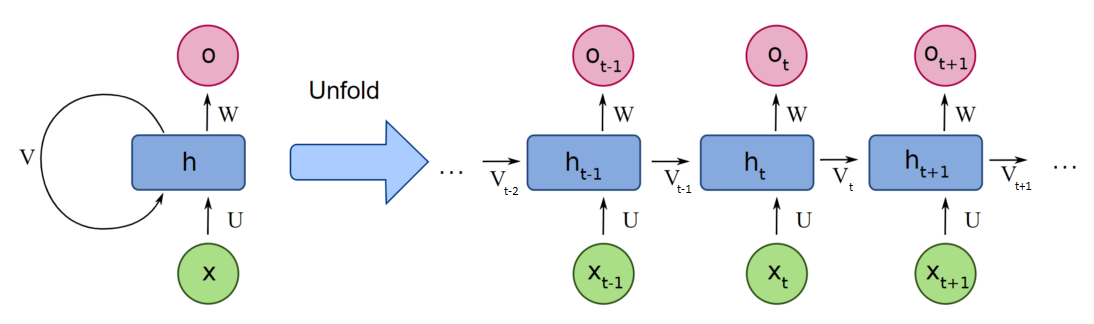
\includegraphics[width=0.6\textwidth]{../images/rnn.png}
    \caption{RNN Architecture}
    \label{fig:rnn}
\end{figure}

The RNN architecture in \Cref{fig:rnn} is a simple RNN. It takes in a sequence of words ($X_i$), and outputs a prediction. The RNN takes input
words one at a time, and passes a hidden state ($V_i$) to the next word. The hidden state contains information about the previous words in the
sequence. At the end of the sequence, the final hidden state of the RNN is fed through a softmax layer to get a probability distribution over the
possible classes.\\
The main problem with RNNs is the affect of short-term memory (long-term dependencies are hard to learn) \cite{vangrad}.
For every new word in the sequence, the RNN `forgets' parts of the
previous words in the sequence. This is because the hidden state is updated by each new word.
\begin{figure}[hbtp]
    \centering
    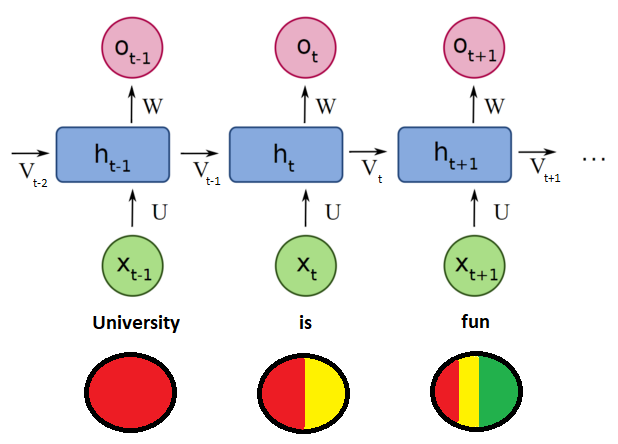
\includegraphics[width=0.6\textwidth]{../images/shortterm-problem.png}
    \caption{Problem with RNNs}
    \label{fig:stm}
\end{figure}

In \cref{fig:stm}, we can see how much each `word' in the sequence affects the hidden state over time. For long sequences,
the hidden state is predominantly affected by the last words in the sequence. This means we lose information about the earlier words
in the sequence. This is caused by vanishing/exploding gradients \cite{vangrad}. Where earlier elements in the sequence have extremely small (or large)
gradients making backpropagation hard to perform \cite{rnn-grad}. This could be a problem with our text classification problem as the key information in the text may be in the
beginning of the sentence. For example: ``Manchester United lost the match 2-1, it was a poor performance but the atmosphere in the
theatre of dreams was astounding.'' The key information in this sentence is that Manchester United lost the match (meaning the text
is about sport). However, this information could be lost due to the short-term memory problem. In the case above it is likely
we classify the text as entertainment due to the later references of `performance' and `theatre'\\
\subsection{Long Short-Term Memory (LSTM) - \cite{lstm}}
The Long Short-Term Memory (LSTM) model was developed in 1997 to solve the short-term memory problem in RNNs \cite{lstm}. It does this by
using 3 memory gates: the input gate, the forget gate and the output gate. These gates perform different functions:
\begin{itemize}
    \item \textbf{Input Gate:} The input gate decides which values from the current input should be added to the cell state.
    \item \textbf{Forget Gate:} The forget gate decides which values from the cell state should be kept.
    \item \textbf{Output Gate:} The output gate decides which values from the cell state should be used to make a prediction.
\end{itemize}
\begin{figure}[hbtp]
    \centering
    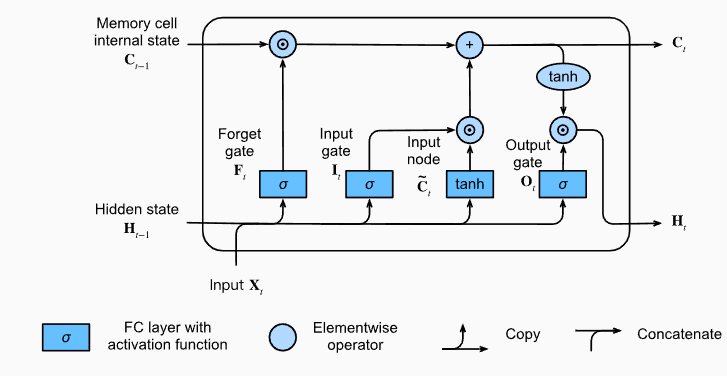
\includegraphics[width=0.6\textwidth]{../images/lstm.png}
    \caption{LSTM Cell Architecture}
    \label{fig:lstm}
\end{figure}
The basic intuition behind how LSTM's solve the vanishing gradient problem is that they use gates to pass on information.
These gates assign a value between 0 and 1 that corresponds to how important the information is. Although this can still
cause a vanishing gradient, it will be the case that if a gradient is vanished then it's input in the forward direction
was not important and therefore the gradient will not be important in the backward direction.\\

LSTM's (as well as RNNs) have another problem: they can only process information in one direction at a time. This means that 
they can only use previous words to understand the current word, or the next words to understand the current word. Bidirectional
versions of these models aim to solve this problem by processing the sequence in both directions at the same time. However, this
is not a perfect solution as it only `learns' the context from both directions and not as a whole. In \cref{sec:transformers}
we will discuss a model that solves this problem.
\subsection{Transformers}
\label{sec:transformers}
\subsubsection{Architecture}
In 2017 Google released a paper called \textit{Attention is all you need} \cite{attention}. This paper introduced the Transformer
architecture.
\newpage
\begin{figure}[hbtp]
    \centering
    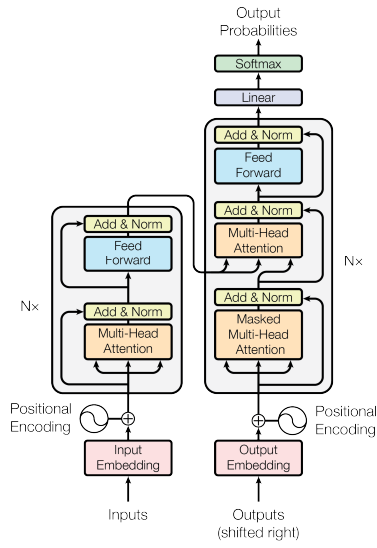
\includegraphics[width=0.6\textwidth]{../images/transformer.png}
    \caption{Transformer Architecture - \cite{attention}}
    \label{fig:transformer}
\end{figure}

\Cref{fig:transformer} shows the architecture of a Transformer model. Focussing on the encoder, the input is passed through
a `Multi-Head Attention' layer. This layer takes in the input and creates a matrix of attention weights. These attention weights
essentially say how much of an impact each word has on each other.
\subsubsection{Self-Attention}
Before looking into Multi-Head Attention, let's discuss Self-Attention.\\
Self-Attention is a Sequence-to-Sequence model that calculates the attention weights between each word in the sequence \cite{attention}. The attention
weights are how important each word is to the other words in the sequence. The attention weights are calculated using 3 vectors:
Query, Key, and Value \cite{attention}. All of these vectors are made from passing the input through a linear layer. Each vector is made using a different
linear layer.
\begin{figure}[hbtp]
    \centering
    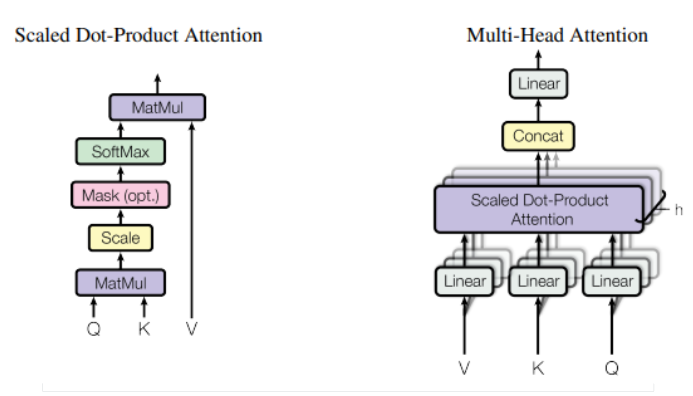
\includegraphics[width=0.6\textwidth]{../images/attention.png}
    \caption{Self-Attention - \cite{attention}}
    \label{fig:self-attention}
\end{figure} 

\Cref{fig:self-attention} shows how the attention weights are calculated. First, the Query and Key vectors are multiplied together.
This is then passed through a softmax layer to convert all weights into probabilities. These probabilities act as the attention weights.
The attention weights are then multiplied by the Value vector to get the final output.
\subsubsection{Multi-Head Attention}
The paper \textit{Attention is all you need} \cite{attention} also introduces the Multi-Head Attention layer. This layer uses self-attention
but splits the Query, Key and Value vectors into multiple heads. Each head calculate the attention weights independently, and their outputs
are concatenated together.
\begin{figure}[hbtp]
    \centering
    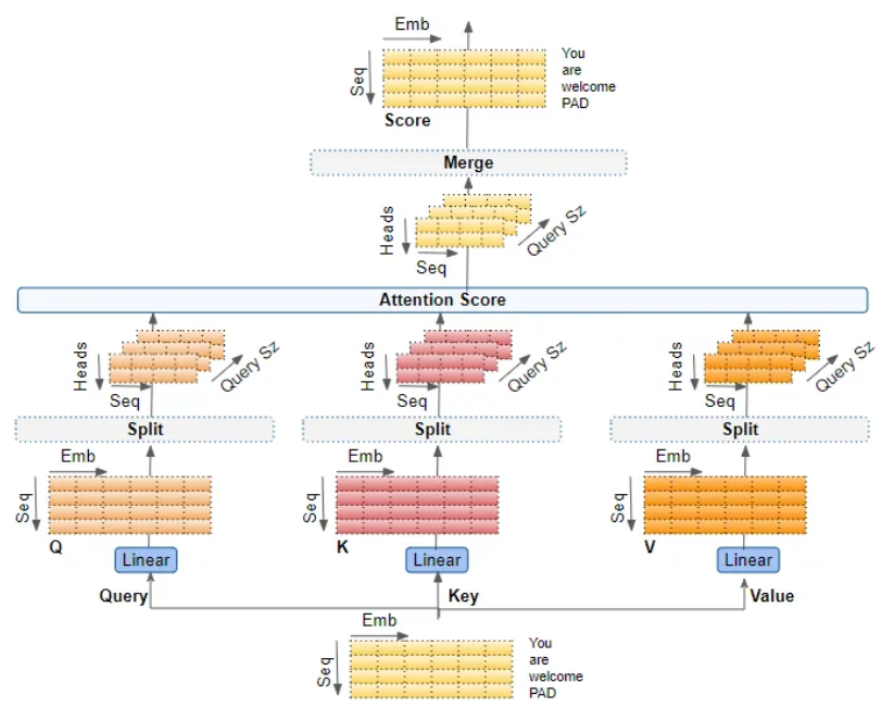
\includegraphics[width=0.6\textwidth]{../images/multi-head-attention.png}
    \caption{Multi-Head Attention}
    \label{fig:multi-head-attention}
\end{figure}

Multi-head attention provides a more stable model throughout training \cite{multi-head-pros}. Although deep single-head attention models have been shown
to be able to outperform shallow multi-head attention models, they require very specific initialisation before training \cite{multi-head-pros}. This is where
multi-head attention models shine. They are able to converge to a good solution without the need for specific initialisation of weights \cite{multi-head-pros}.
\subsection{Bidirectional Encoder Representation of Transformers (BERT) - \cite{bert}}
BERT is an acronym for Bidirectional Encoder Representations from Transformers. It's architecture uses several Transformer encoders
put together. Transformers make use of self-attention to learn contextual representation of words. This solves the problem
discussed in \Cref{sec:RNN} where the RNNs only look at the previous words in the sentence, or both directions independently.
\begin{figure}[hbtp]
    \centering
    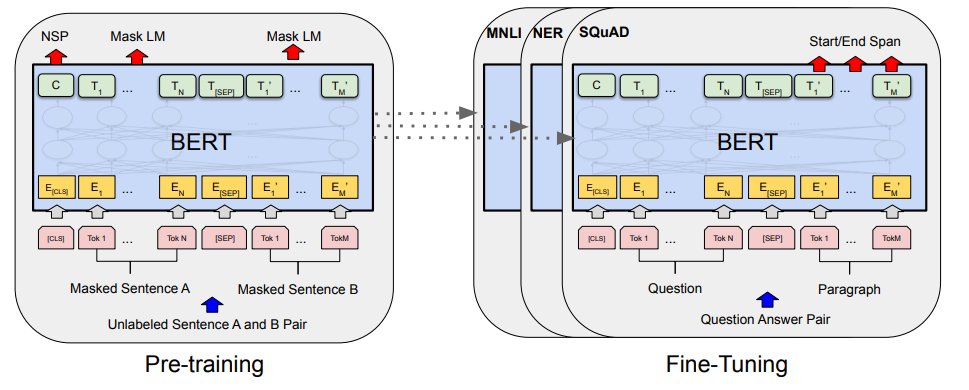
\includegraphics[width=0.6\textwidth]{../images/bert.png}
    \caption{BERT Architecture}
    \label{fig:bert}
\end{figure}

A BERT classification model is trained in 2 steps: pre-training and fine-tuning. The pre-training step is done on a large corpus
by Google. The fine-tuning step is done on a smaller dataset specific to the task at hand.

\subsubsection{pre-training}
The pre-training step of the BERT model consists of learning 2 objectives: masked language modelling (MLM) and next sentence prediction
(NSP).\\
\textbf{Masked Language Modelling (MLM)} is a task where the model is given a sentence with some words masked out. The model is then
expected to predict the masked words.\\
\textbf{Next Sentence Prediction (NSP)} is a task where the model is given 2 sentences, a and b. The model is then expected to predict
whether sentence b is the next sentence following a.\\\\

The pre-training step is done on a large corpus of unlabelled data. This makes it easy to train the model, as it does not require
collecting a large amount of labelled data. Using Transformers makes the model more efficient, as it can process the entire sentence
at once instead of processing the sentence word by word.

\subsubsection{fine-tuning}
To use BERT for our task of topic classification, we need to fine-tune the model using a labelled dataset - posts labelled with the
corresponding topic they belong to (as figured out in \Cref{sec:supervised-learning}).\\
Before fine-tuning, the model needs a final output layer to be added. This output layer will be a linear layer with x neurons, where
x is the number of topics (so currently 23). The fine-tuning step is trained using categorical cross-entropy loss, and the Adam optimizer.
The model is trained for 6 epochs, with a batch size of 32. The model is then evaluated on the test set, achieving an accuracy
of $\approx 42\%$. Please refer to \Cref{ch:evaluation} for a more detailed analysis of the model's performance.

\subsection{Robustly Optimised BERT Approach (RoBERTa) - \cite{DBLP:journals/corr/abs-1907-11692}}
RoBERTa is a variant of BERT that is more efficient and robust. It uses the same architecture as BERT, but with some modifications to 
the pre-training step. RoBERTa only performs the masked language modelling task, and does not perform the next sentence prediction task.
On top of this, RoBERTa uses dynamic masking, where during runtime the model randomly masks out words in the sentence, instead of
masking out words statically (masking the same words for a given sentence). The paper introducing RoBERTa also analysed the effect
of the pre-training corpus size, batch size, and number of training steps on the model's performance. They found ``t performance can be substantially
improved by training the model longer, with bigger batches over more data'' \cite{DBLP:journals/corr/abs-1907-11692}\\
Hence the pre-training of RoBERTa was done on a larger corpus of text than BERT. This improved the model's performance.
\begin{figure}[hbtp]
    \centering
    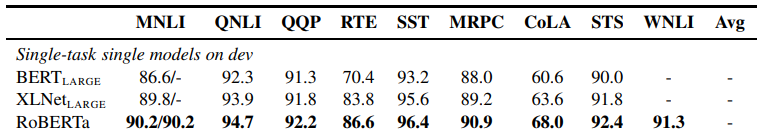
\includegraphics[width=0.6\textwidth]{../images/roberta-tasks.png}
    \caption{Comparing RoBERTa and BERT - \cite{DBLP:journals/corr/abs-1907-11692}}
    \label{fig:bertcomproberta}
\end{figure}

\Cref{fig:bertcomproberta} shows how RoBERTa performs better than BERT on most NLP benchmark tests. This led to RoBERTa being tested for
this project. RoBERTa was fine-tuned using the same method as BERT, and achieved an accuracy of $\approx 71\%$ on the test set.
Evaluation of the model is discussed in \Cref{ch:evaluation}.